% Options for packages loaded elsewhere
\PassOptionsToPackage{unicode}{hyperref}
\PassOptionsToPackage{hyphens}{url}
%
\documentclass[
]{book}
\usepackage{amsmath,amssymb}
\usepackage{iftex}
\ifPDFTeX
  \usepackage[T1]{fontenc}
  \usepackage[utf8]{inputenc}
  \usepackage{textcomp} % provide euro and other symbols
\else % if luatex or xetex
  \usepackage{unicode-math} % this also loads fontspec
  \defaultfontfeatures{Scale=MatchLowercase}
  \defaultfontfeatures[\rmfamily]{Ligatures=TeX,Scale=1}
\fi
\usepackage{lmodern}
\ifPDFTeX\else
  % xetex/luatex font selection
\fi
% Use upquote if available, for straight quotes in verbatim environments
\IfFileExists{upquote.sty}{\usepackage{upquote}}{}
\IfFileExists{microtype.sty}{% use microtype if available
  \usepackage[]{microtype}
  \UseMicrotypeSet[protrusion]{basicmath} % disable protrusion for tt fonts
}{}
\makeatletter
\@ifundefined{KOMAClassName}{% if non-KOMA class
  \IfFileExists{parskip.sty}{%
    \usepackage{parskip}
  }{% else
    \setlength{\parindent}{0pt}
    \setlength{\parskip}{6pt plus 2pt minus 1pt}}
}{% if KOMA class
  \KOMAoptions{parskip=half}}
\makeatother
\usepackage{xcolor}
\usepackage{color}
\usepackage{fancyvrb}
\newcommand{\VerbBar}{|}
\newcommand{\VERB}{\Verb[commandchars=\\\{\}]}
\DefineVerbatimEnvironment{Highlighting}{Verbatim}{commandchars=\\\{\}}
% Add ',fontsize=\small' for more characters per line
\usepackage{framed}
\definecolor{shadecolor}{RGB}{248,248,248}
\newenvironment{Shaded}{\begin{snugshade}}{\end{snugshade}}
\newcommand{\AlertTok}[1]{\textcolor[rgb]{0.94,0.16,0.16}{#1}}
\newcommand{\AnnotationTok}[1]{\textcolor[rgb]{0.56,0.35,0.01}{\textbf{\textit{#1}}}}
\newcommand{\AttributeTok}[1]{\textcolor[rgb]{0.13,0.29,0.53}{#1}}
\newcommand{\BaseNTok}[1]{\textcolor[rgb]{0.00,0.00,0.81}{#1}}
\newcommand{\BuiltInTok}[1]{#1}
\newcommand{\CharTok}[1]{\textcolor[rgb]{0.31,0.60,0.02}{#1}}
\newcommand{\CommentTok}[1]{\textcolor[rgb]{0.56,0.35,0.01}{\textit{#1}}}
\newcommand{\CommentVarTok}[1]{\textcolor[rgb]{0.56,0.35,0.01}{\textbf{\textit{#1}}}}
\newcommand{\ConstantTok}[1]{\textcolor[rgb]{0.56,0.35,0.01}{#1}}
\newcommand{\ControlFlowTok}[1]{\textcolor[rgb]{0.13,0.29,0.53}{\textbf{#1}}}
\newcommand{\DataTypeTok}[1]{\textcolor[rgb]{0.13,0.29,0.53}{#1}}
\newcommand{\DecValTok}[1]{\textcolor[rgb]{0.00,0.00,0.81}{#1}}
\newcommand{\DocumentationTok}[1]{\textcolor[rgb]{0.56,0.35,0.01}{\textbf{\textit{#1}}}}
\newcommand{\ErrorTok}[1]{\textcolor[rgb]{0.64,0.00,0.00}{\textbf{#1}}}
\newcommand{\ExtensionTok}[1]{#1}
\newcommand{\FloatTok}[1]{\textcolor[rgb]{0.00,0.00,0.81}{#1}}
\newcommand{\FunctionTok}[1]{\textcolor[rgb]{0.13,0.29,0.53}{\textbf{#1}}}
\newcommand{\ImportTok}[1]{#1}
\newcommand{\InformationTok}[1]{\textcolor[rgb]{0.56,0.35,0.01}{\textbf{\textit{#1}}}}
\newcommand{\KeywordTok}[1]{\textcolor[rgb]{0.13,0.29,0.53}{\textbf{#1}}}
\newcommand{\NormalTok}[1]{#1}
\newcommand{\OperatorTok}[1]{\textcolor[rgb]{0.81,0.36,0.00}{\textbf{#1}}}
\newcommand{\OtherTok}[1]{\textcolor[rgb]{0.56,0.35,0.01}{#1}}
\newcommand{\PreprocessorTok}[1]{\textcolor[rgb]{0.56,0.35,0.01}{\textit{#1}}}
\newcommand{\RegionMarkerTok}[1]{#1}
\newcommand{\SpecialCharTok}[1]{\textcolor[rgb]{0.81,0.36,0.00}{\textbf{#1}}}
\newcommand{\SpecialStringTok}[1]{\textcolor[rgb]{0.31,0.60,0.02}{#1}}
\newcommand{\StringTok}[1]{\textcolor[rgb]{0.31,0.60,0.02}{#1}}
\newcommand{\VariableTok}[1]{\textcolor[rgb]{0.00,0.00,0.00}{#1}}
\newcommand{\VerbatimStringTok}[1]{\textcolor[rgb]{0.31,0.60,0.02}{#1}}
\newcommand{\WarningTok}[1]{\textcolor[rgb]{0.56,0.35,0.01}{\textbf{\textit{#1}}}}
\usepackage{longtable,booktabs,array}
\usepackage{calc} % for calculating minipage widths
% Correct order of tables after \paragraph or \subparagraph
\usepackage{etoolbox}
\makeatletter
\patchcmd\longtable{\par}{\if@noskipsec\mbox{}\fi\par}{}{}
\makeatother
% Allow footnotes in longtable head/foot
\IfFileExists{footnotehyper.sty}{\usepackage{footnotehyper}}{\usepackage{footnote}}
\makesavenoteenv{longtable}
\usepackage{graphicx}
\makeatletter
\def\maxwidth{\ifdim\Gin@nat@width>\linewidth\linewidth\else\Gin@nat@width\fi}
\def\maxheight{\ifdim\Gin@nat@height>\textheight\textheight\else\Gin@nat@height\fi}
\makeatother
% Scale images if necessary, so that they will not overflow the page
% margins by default, and it is still possible to overwrite the defaults
% using explicit options in \includegraphics[width, height, ...]{}
\setkeys{Gin}{width=\maxwidth,height=\maxheight,keepaspectratio}
% Set default figure placement to htbp
\makeatletter
\def\fps@figure{htbp}
\makeatother
\setlength{\emergencystretch}{3em} % prevent overfull lines
\providecommand{\tightlist}{%
  \setlength{\itemsep}{0pt}\setlength{\parskip}{0pt}}
\setcounter{secnumdepth}{5}
\usepackage{booktabs}
\ifLuaTeX
  \usepackage{selnolig}  % disable illegal ligatures
\fi
\usepackage[]{natbib}
\bibliographystyle{apalike}
\IfFileExists{bookmark.sty}{\usepackage{bookmark}}{\usepackage{hyperref}}
\IfFileExists{xurl.sty}{\usepackage{xurl}}{} % add URL line breaks if available
\urlstyle{same}
\hypersetup{
  pdftitle={R for Geoscience},
  pdfauthor={Shuxin Ji},
  hidelinks,
  pdfcreator={LaTeX via pandoc}}

\title{R for Geoscience}
\author{Shuxin Ji}
\date{2023-08-13}

\begin{document}
\maketitle

{
\setcounter{tocdepth}{1}
\tableofcontents
}
\hypertarget{about}{%
\chapter*{About}\label{about}}
\addcontentsline{toc}{chapter}{About}

你好,这里是shuxin对R在地理数据处理方面能力的第一次尝试。 博士入学时,导师告诉我最好还是要掌握一门语言来对地理数据进行处理,因为在日后的工作中 总会遇到大体量数据而不能通过手工完成,所以这是写下这本参考书目的原因之一。在未接触R之前,我都是通过桌面软件Arcgis,Qgis,ENVI,SNAP完成地理数据的查找,下载,预处理等工作,这种方法的好处就在于每一步都是所见即所得,自己心中可以清楚的预计每一步之后的结果大概是怎样的,但缺点也非常明显,一旦某一步操作出现了纰漏就可能对最终处理结果产生影响,进而导致结果的不可信,每当这时就需要从头开始梳理,重复数据的处理过程,这对我的工作积极性造成非常大的打击,我相信经历过以上过程的你一定深有体会。

本书的重点主要放在地理工作中可能出现的问题上,也可以算作对我博士研究阶段所遇到问题的总结。 期间所用到的主要工具是R,在这里我不会给大家展示各种绚丽的代码,只需要大家跟随本书的思路,一步步 实践下来,当你能轻松的应对本书所描述的各类问题时,我相信你就已经是一位合格的地理工作者了。

在我的学习期间,导师的日常工作非常繁忙,一年可以见到他的次数屈指可数,因为他每天除了要应对科研工作外,还要兼顾本科生和研究生的教学工作,所以每次见到他时都很疲惫,因为总会因为学生们的基础不同,而让他的教学没有办法有的放矢,为了避免出现类似状况,在此记录下要成为一名地理科研工作者所需要具备的基本条件。

此书行文并不会像市面上传统的书籍讳莫如深,相反我是一个自由散漫的人,追求以最通俗易懂的话让你明白我想表达的意思,当然如果这让我的硕导看到的话肯定会说我不严谨或者大白话,但文字的意义不就是在此吗?所以不要害怕继续看下去,仔细读一下,动手操作一下,有问题就问一下(囿于本人才疏学浅,无论在行文亦或是代码部分可能会出现错误,请您不要吝惜您的指正,欢迎在github主页提出问题,感谢您啦),一切都会变的简单起来。

回想过去几年的学习生涯,往往会被一个个小问题卡住,其实后来回头看看也就是很简单的一行代码,一个鼠标点击,仅此而已。然而当局者迷,当自己孤身一人想要实现一个东西而身边又没有人可以求教时,那种孤独、痛苦真的会让自己变得不开心甚至抑郁,我懂你的。而当导师或者同学给你指了路或者给你演示了一边,通过了这个小关卡,瞬间觉得欣喜若狂,仿佛觉得我又行了,是啊,科研工作就是这样,总是让人又爱又恨。

学会提问也是很重要的,我认为最有效的方法就是有一个了解甚至经历过你所在研究方向的人给你\texttt{打个样},这样你很快就能模仿着上手,开始你的工作。现实中很难找到这样的人,导师或者师兄师姐都很忙,可能处于不好意思,也就不想继续问下去了,然后又回到了自己emo的死循环中。本书会重点告诉你如果你不知道怎么办的时候应该做什么,阅读完本书后你一定会变得更加自信!

作者认为要成为一名优秀的地理数据处理工作者,需要具备以下素质,

\begin{itemize}
\tightlist
\item
  掌握地理学的基础知识,包括地球科学、地理信息科学、地图学、地理统计学等。
\item
  掌握数据分析技能,例如统计分析、数据可视化、机器学习等。
\item
  熟悉并熟练掌握地理数据处理工具ArcGIS、QGIS、R、Python或Javascript等。
\item
  有Linux系统使用经验,能使用shell对系统进行监测。
\end{itemize}

\hypertarget{ux8bfeux7a0bux5b89ux6392}{%
\section*{\texorpdfstring{\textbf{课程安排}}{课程安排}}\label{ux8bfeux7a0bux5b89ux6392}}
\addcontentsline{toc}{section}{\textbf{课程安排}}

\hypertarget{practice}{%
\section*{\texorpdfstring{\textbf{practice}}{practice}}\label{practice}}
\addcontentsline{toc}{section}{\textbf{practice}}

\hypertarget{part-ux57faux7840ux77e5ux8bc6}{%
\part{基础知识}\label{part-ux57faux7840ux77e5ux8bc6}}

\hypertarget{rux8bedux8a00ux5165ux95e8}{%
\chapter{R语言入门}\label{rux8bedux8a00ux5165ux95e8}}

\hypertarget{what-is-r}{%
\section{What is R?}\label{what-is-r}}

R 是一种用于统计计算和图形的编程语言和环境。 它由新西兰奥克兰大学的 Ross Ihaka 和 Robert Gentleman 在 20 世纪 90 年代中期开发。 R 在 GNU 通用公共许可证下免费提供,它已成为统计学家、数据科学家和研究人员中的流行工具。

R 提供了多种统计和图形技术,包括线性和非线性建模、时间序列分析、聚类等。 它还拥有来自世界各地的用户贡献的大量软件包,进一步扩展了它的功能。 这些包可以很容易地安装并加载到 R 中以用于特定任务。

R 有一个命令行界面,但也有几个集成开发环境 (IDE) 可用,例如 RStudio,它们提供了更加用户友好的界面。 R 通常与其他工具(如 SQL、Python 或 Excel)结合使用以进行数据操作和分析。

\hypertarget{why-r}{%
\section{Why R?}\label{why-r}}

R 是统计计算和数据分析的流行选择,原因如下:

\begin{itemize}
\item
  开源免费:R 是一个开源软件,这意味着任何人都可以免费下载、使用和修改它。 这使得包括学生、研究人员和专业人士在内的大量用户可以访问它。
\item
  强大的统计计算:R旨在处理复杂的统计计算和图形,使其适用于范围广泛的数据分析任务。 它提供了大量内置统计函数和包,涵盖范围广泛的技术,从基本的描述性统计到高级建模和机器学习算法。
\item
  庞大的用户社区:R 拥有庞大而活跃的用户社区,这意味着有大量的资源和支持可供用户使用。 有许多在线论坛、教程和书籍可帮助用户学习和解决问题。
\item
  可重复研究:R 提供了创建可重复研究的工具,这意味着可以记录整个数据分析过程并与他人共享,从而使其他人更容易复制分析并验证结果。
\item
  与其他工具集成:R 可以轻松与其他工具集成,例如 SQL 数据库、Python 和 Excel,从而更轻松地处理以不同格式存储的数据。
\end{itemize}

总的来说,R 是一种强大而灵活的数据分析工具,广泛应用于学术界、研究界和工业界。 它的流行是由于它的可访问性、功能以及支持它的庞大的用户和开发人员社区。

\hypertarget{ux5b89ux88c5ux4e0eux914dux7f6e}{%
\section{安装与配置}\label{ux5b89ux88c5ux4e0eux914dux7f6e}}

\hypertarget{ux4e0bux8f7dux5e76ux5b89ux88c5r}{%
\subsection{下载并安装R}\label{ux4e0bux8f7dux5e76ux5b89ux88c5r}}

R是一种自由软件,您可以从\href{https://www.r-project.org}{R官方网站}下载R的最新版本。根据您的操作系统选择下载对应的版本,然后按照提示安装即可。国内用户推荐使用清华源进行下载。

\hypertarget{ux5b89ux88c5rstudio}{%
\subsection{安装RStudio}\label{ux5b89ux88c5rstudio}}

RStudio是一款用于R编程的集成开发环境,它可以提供更方便的R编程和数据分析工具。您可以从\href{https://www.rstudio.com/}{官方网站}下载最新的RStudio Desktop版,并安装在您的计算机上。如果您是Max OS或Linux用户,请选择相对应的安装包。

\hypertarget{rstudioux914dux7f6e}{%
\subsection{Rstudio配置}\label{rstudioux914dux7f6e}}

这一步更多的是对自己的生产环境进行配置,可以根据个人喜好进行更改,这里不再赘述\\
请参考:\href{https://www.jianshu.com/p/d5360a387311}{软件安装配置------Rstudio配置}

\hypertarget{ux5b89ux88c5ux5e38ux7528ux7684rux5305}{%
\subsection{安装常用的R包}\label{ux5b89ux88c5ux5e38ux7528ux7684rux5305}}

R包是R语言的扩展程序,它们包含了许多有用的函数和工具,可以方便地完成许多数据处理和分析任务。在RStudio中,您可以使用以下代码安装一些常用的R包:
请参考:\href{https://www.jianshu.com/p/5a066d66d3d3}{软件安装配置------R包的使用}
- 安装单个包

\begin{Shaded}
\begin{Highlighting}[]
\FunctionTok{install.packages}\NormalTok{(}\StringTok{"terra"}\NormalTok{)}
\end{Highlighting}
\end{Shaded}

\begin{itemize}
\tightlist
\item
  安装多个包
\end{itemize}

\begin{Shaded}
\begin{Highlighting}[]
\FunctionTok{install.packages}\NormalTok{(}\FunctionTok{c}\NormalTok{(}\StringTok{"terra"}\NormalTok{, }\StringTok{"pacman"}\NormalTok{, }\StringTok{"tidyverse"}\NormalTok{, }\StringTok{"leaflet"}\NormalTok{))}
\end{Highlighting}
\end{Shaded}

\begin{itemize}
\tightlist
\item
  上述方法虽可以一次安装多个包,但还需要逐个加载,\texttt{pacman}包的好处是可以一次加载多个包,若某个包没有安装则自动安装并加载
\end{itemize}

\begin{Shaded}
\begin{Highlighting}[]
\FunctionTok{ifelse}\NormalTok{(}\SpecialCharTok{!}\StringTok{"pacman"} \SpecialCharTok{\%in\%} \FunctionTok{installed.packages}\NormalTok{(), }\FunctionTok{install.packages}\NormalTok{(}\StringTok{"pacman"}\NormalTok{),}
       \FunctionTok{library}\NormalTok{(pacman))}
\FunctionTok{p\_load}\NormalTok{(terra, tidyverse, leaflet)}
\end{Highlighting}
\end{Shaded}

{Attention, Please!}\\
Please do not use any {Chinese charactor(中文字符)} to set your path!

\hypertarget{ux6ce8ux91ca-comments}{%
\section{注释 comments}\label{ux6ce8ux91ca-comments}}

R在执行代码时会忽略注释,它们不会影响程序的输出或行为。在R中注释符号\texttt{\#}键,也支持多行注释,选中需要注释的多行内容,按下快捷键为\texttt{Ctrl+Shift+C}即可。\\
为你的代码添加注释有以下几个好处:

\begin{itemize}
\tightlist
\item
  记录代码:注释可用于解释代码的作用,为什么以某种方式编写代码,或为未来的读者提供上下文。 好的注释可以使代码更易于理解、维护和修改。\\
\item
  协作:如果您正在与其他人一起处理一个项目,评论可以帮助其他团队成员理解您的代码并使他们更容易与您协作。\\
\item
  调试:当您的代码遇到问题时,注释可以帮助您隔离问题并更快地找到解决方案。\\
\item
  请养成良好的代码书写习惯,提高代码可读性。
\end{itemize}

\begin{Shaded}
\begin{Highlighting}[]
\DecValTok{1} \SpecialCharTok{+} \DecValTok{2}    \CommentTok{\# this is use to sum 1 and 2}
\end{Highlighting}
\end{Shaded}

\hypertarget{ux5185ux7f6eux51fdux6570}{%
\section{内置函数}\label{ux5185ux7f6eux51fdux6570}}

R内置了很多的基础函数,像求和、比较大小等等,在我刚接触R时非常疑惑,除了这些常见的函数外,R到底内置了多少函数呢?有的时候自己傻傻的写函数想要实现某些功能,到头来却发现R中有现成的可以用,真是浪费时间和精力。你可以在\href{https://stat.ethz.ch/R-manual/R-devel/library/base/html/00Index.html}{The R Base Package}中找到答案。

\hypertarget{ux6570ux636eux7ed3ux6784}{%
\chapter{数据结构}\label{ux6570ux636eux7ed3ux6784}}

\hypertarget{vectorux5411ux91cf}{%
\section{Vector(向量)}\label{vectorux5411ux91cf}}

Vector是R中的一种基础数据结构,它包含相同类型的元素。数据类型可以是逻辑、整数、双精度、字符、复杂或原始。

举个例子,现在我们有1到5,5个整数,想要把他们组成一个向量应该怎么操作呢?

\begin{Shaded}
\begin{Highlighting}[]
\NormalTok{x }\OtherTok{\textless{}{-}} \FunctionTok{c}\NormalTok{(}\DecValTok{1}\NormalTok{,}\DecValTok{2}\NormalTok{,}\DecValTok{3}\NormalTok{,}\DecValTok{4}\NormalTok{,}\DecValTok{5}\NormalTok{)}
\NormalTok{x}
\CommentTok{\#\textgreater{} [1] 1 2 3 4 5}
\end{Highlighting}
\end{Shaded}

这里我们用\texttt{c()}函数来把1,2,3,4,5组合起来,然后通过\texttt{\textless{}-}这个符号把这个值赋给\texttt{x},这样就把一个简单的向量给构建完成了。请仔细体会这句话的涵义,先把第一要做的事情\texttt{组合1,2,3,4,5}完成,然后再赋值给一个变量\texttt{x},请牢记这里的思路,这对后续R的运算是十分有帮助的。
当然了,大家刚接触R心里肯定会有疑问,这个\texttt{c()}到底是干啥的,这个函数除了这么简单的组合起一个向量,还能做点别的不?这里就讲到一个非常重要的点,即查阅!学东西得会学,不能说是看了这本书讲了这样做,你能模仿下来,换本书举了个不一样的例子你就懵了,那相当于啥也没学,净看作者耍贫嘴去了。所以当对一个函数不了解或者想要刨根问底时,\texttt{??}小问号就排上用场了,我们在\texttt{Console}中输入\texttt{??c()},右侧的Help页面就会弹出来关于该函数的帮助文档,请记住任何人都不会比函数开发者更加了解自己的函数是干啥的,同理以后若遇到新的函数你就知道该怎么做了。

当然了,R也是一门语言,和其他语言一样,也是各种符号骚操作满天飞,不过不必惊慌,常用的也就那么几个,大神们也只是用的多了,脑子里记得的比我们更多一些,你与大神的差距真的就只是练的用的太少了(其实大神也是需要google的)。那这里就介绍本书的第一个符号\texttt{:},中文里我们用作冒号,在R中我们可以理解为\texttt{到},打个样给你看看,还是以上面的构造向量为例,

\begin{Shaded}
\begin{Highlighting}[]
\NormalTok{x }\OtherTok{\textless{}{-}} \FunctionTok{c}\NormalTok{(}\DecValTok{1}\SpecialCharTok{:}\DecValTok{5}\NormalTok{)}
\NormalTok{x}
\CommentTok{\#\textgreater{} [1] 1 2 3 4 5}
\end{Highlighting}
\end{Shaded}

开头我们讲了,vector有很多不同的类型,那么我们在看到一个向量时怎么去看看它到底是啥类型呢?这时候需要用到\texttt{typeof()}这个函数,

\begin{Shaded}
\begin{Highlighting}[]
\FunctionTok{typeof}\NormalTok{(x)}
\CommentTok{\#\textgreater{} [1] "integer"}
\end{Highlighting}
\end{Shaded}

除了类型之外,向量还有另外一个十分重要的特征就是长度(length),\texttt{length()}可以用来查看向量长度,

\begin{Shaded}
\begin{Highlighting}[]
\FunctionTok{length}\NormalTok{(x)}
\CommentTok{\#\textgreater{} [1] 5}
\end{Highlighting}
\end{Shaded}

自己动手输入数值还是挺麻烦的,R中的\texttt{seq()}可以帮助我们更快的创造一个向量,打个样,

\begin{Shaded}
\begin{Highlighting}[]
\FunctionTok{seq}\NormalTok{(}\DecValTok{1}\NormalTok{, }\DecValTok{9}\NormalTok{, }\FloatTok{0.5}\NormalTok{)}
\CommentTok{\#\textgreater{}  [1] 1.0 1.5 2.0 2.5 3.0 3.5 4.0 4.5 5.0 5.5 6.0 6.5 7.0 7.5}
\CommentTok{\#\textgreater{} [15] 8.0 8.5 9.0}
\end{Highlighting}
\end{Shaded}

很神奇有没有,爱心算的你很快就知道了这行代码的意思是从1到9每间隔0.5输出一个值,但是为啥要这3个数字这么排列呢?这时候就得小问号\texttt{??}上场了,在Console中输入\\
\texttt{??seq}\strut \\
此时看到右侧\texttt{Help}界面的你心里默默念了一句什么鬼,能理解,换谁谁也蒙圈,啥呀都是,乱七八糟的这,莫慌,仔细看是不是这些蓝色的都有一个规律,就是里面都有一个\texttt{::}这个符号,两个小冒号连在一起,啥意思呢?\texttt{包::函数},\texttt{package::function},第一个就是cli这个包里的ansi\_regex函数的意思,第二个就是cli这个包里的ansi\_strip函数的意思。所以我们要找的应该是\texttt{base::seq}这个函数,为啥呢,看后面那句解释啊,sequence generation,这不写的生成随机数嘛。\\
点击进去以后一看还是有点懵,莫慌,一步步来,首先看\texttt{Description}知道这个函数是用来构造随机数的。然后\texttt{Usage},\texttt{seq(...)}这个的意思就是告诉你,你要用我生成随机数,格式就是这样的\texttt{seq}开头,跟着个\texttt{()},括号里呢就要开始放条件了,都有啥条件呢,咱们来看下面的\texttt{Arguments},\texttt{from}说白了就是从几开始,\texttt{to}就是到哪个数结束,\texttt{by}就是前面俩数的间隔是多少,就这么简单。看到这之后心里就有个初步印象了,然后蹦过中间段直接到最后的\texttt{Example},直接贴心的给你放上几个例子,每个开发者都是生怕你不会用我的包啊,就差现场给你讲咋用了,于我而言也是一样的,把例子每一个都运行一遍,看看每一步都产生了啥结果,运行几次然后再回头对照上面的解释文档,也就差不多掌握了这个函数的基本用法了。

看到这我们再来放上其他几个数据类型的vector,

\begin{Shaded}
\begin{Highlighting}[]
\CommentTok{\# Vector of logical values}
\NormalTok{log\_values }\OtherTok{\textless{}{-}} \FunctionTok{c}\NormalTok{(}\ConstantTok{TRUE}\NormalTok{, }\ConstantTok{FALSE}\NormalTok{, }\ConstantTok{TRUE}\NormalTok{, }\ConstantTok{FALSE}\NormalTok{)}

\NormalTok{log\_values}
\CommentTok{\#\textgreater{} [1]  TRUE FALSE  TRUE FALSE}
\end{Highlighting}
\end{Shaded}

忘了讲,\texttt{\#}井号键这个小符号挺好用,干啥的呢,注释掉一句话,说人话就是我这句话写在这了,但R你别给我运行,这句话就是提醒自己下面的代码是要干啥的,防止自己以后再回来看到自己写的东西一整个懵住,现在我也一直保持这个习惯,因为每天看的东西很多,回看过去的东西时经常会忘记当时为啥要这么写,还是挺有用处的,好记性不如烂笔头嘛!
回到正文,上面的就是所谓的逻辑型向量,同理我们再构造一个字符型的,

\begin{Shaded}
\begin{Highlighting}[]
\NormalTok{fruits }\OtherTok{\textless{}{-}} \FunctionTok{c}\NormalTok{(}\StringTok{"beijing"}\NormalTok{, }\StringTok{"shanghai"}\NormalTok{, }\StringTok{"guangzhou"}\NormalTok{, }\StringTok{"shenzhen"}\NormalTok{, }\StringTok{"xianggang"}\NormalTok{, }\StringTok{"50"}\NormalTok{)}
\NormalTok{fruits}
\CommentTok{\#\textgreater{} [1] "beijing"   "shanghai"  "guangzhou" "shenzhen" }
\CommentTok{\#\textgreater{} [5] "xianggang" "50"}
\end{Highlighting}
\end{Shaded}

字符型的呢就要注意要给每一个单词或者数字加上英文双引号。

在实际应用中,有时候我们只想用一个向量中的某个或某几个元素,这时候该咋办呢?这里介绍一种方法,\texttt{{[}{]}},中括号,英文\texttt{brackets},比如我要把fruits中的\texttt{"beijing"}和\texttt{"shenzhen"}拿出来,

\begin{Shaded}
\begin{Highlighting}[]
\NormalTok{fruits[}\FunctionTok{c}\NormalTok{(}\DecValTok{1}\NormalTok{,}\DecValTok{4}\NormalTok{)]}
\CommentTok{\#\textgreater{} [1] "beijing"  "shenzhen"}
\end{Highlighting}
\end{Shaded}

前四个:

\begin{Shaded}
\begin{Highlighting}[]
\NormalTok{fruits[}\DecValTok{1}\SpecialCharTok{:}\DecValTok{4}\NormalTok{]}
\CommentTok{\#\textgreater{} [1] "beijing"   "shanghai"  "guangzhou" "shenzhen"}
\end{Highlighting}
\end{Shaded}

如果想要选取除了\texttt{"beijing}以外的所有元素,这时候可以用减号,

\begin{Shaded}
\begin{Highlighting}[]
\NormalTok{fruits[}\SpecialCharTok{{-}}\DecValTok{1}\NormalTok{]}
\CommentTok{\#\textgreater{} [1] "shanghai"  "guangzhou" "shenzhen"  "xianggang"}
\CommentTok{\#\textgreater{} [5] "50"}
\end{Highlighting}
\end{Shaded}

注意这里的数字代表的是各个元素所在位置。

当然了,对向量内元素进行排序也是可以的,遵循原则就是从小到大或者按照首字母排序,函数为\texttt{sort},

\begin{Shaded}
\begin{Highlighting}[]
\NormalTok{fruits }\OtherTok{\textless{}{-}} \FunctionTok{c}\NormalTok{(}\StringTok{"beijing"}\NormalTok{, }\StringTok{"shanghai"}\NormalTok{, }\StringTok{"guangzhou"}\NormalTok{, }\StringTok{"shenzhen"}\NormalTok{, }\StringTok{"xianggang"}\NormalTok{)}
\NormalTok{numbers }\OtherTok{\textless{}{-}} \FunctionTok{c}\NormalTok{(}\DecValTok{13}\NormalTok{, }\DecValTok{3}\NormalTok{, }\DecValTok{5}\NormalTok{, }\DecValTok{7}\NormalTok{, }\DecValTok{20}\NormalTok{, }\DecValTok{2}\NormalTok{)}

\FunctionTok{sort}\NormalTok{(fruits)  }\CommentTok{\# Sort a string}
\CommentTok{\#\textgreater{} [1] "beijing"   "guangzhou" "shanghai"  "shenzhen" }
\CommentTok{\#\textgreater{} [5] "xianggang"}
\FunctionTok{sort}\NormalTok{(numbers) }\CommentTok{\# Sort numbers}
\CommentTok{\#\textgreater{} [1]  2  3  5  7 13 20}
\end{Highlighting}
\end{Shaded}

\hypertarget{listsux5217ux8868}{%
\section{Lists(列表)}\label{listsux5217ux8868}}

R 中的列表可以在其中包含许多不同的数据类型,列表是有序且可变的数据集合。啥意思呢?
说人话就是甭管啥类型数据都往里搁就完了,要创建列表,使用\texttt{list()}函数:打个样,

\begin{Shaded}
\begin{Highlighting}[]
\NormalTok{thislist }\OtherTok{\textless{}{-}} \FunctionTok{list}\NormalTok{(}
  \AttributeTok{a =} \FunctionTok{c}\NormalTok{(}\StringTok{"shanghai"}\NormalTok{, }\StringTok{"beijing"}\NormalTok{, }\StringTok{"cherry"}\NormalTok{),}
  \AttributeTok{b =} \FunctionTok{c}\NormalTok{(}\DecValTok{1}\NormalTok{,}\DecValTok{2}\NormalTok{,}\DecValTok{5}\NormalTok{,}\DecValTok{6}\NormalTok{,}\DecValTok{7}\NormalTok{,}\DecValTok{9}\NormalTok{),}
  \AttributeTok{c =} \FunctionTok{c}\NormalTok{(}\ConstantTok{TRUE}\NormalTok{, }\ConstantTok{FALSE}\NormalTok{, }\ConstantTok{TRUE}\NormalTok{)}
\NormalTok{)}
\CommentTok{\# Print the list}
\NormalTok{thislist}
\CommentTok{\#\textgreater{} $a}
\CommentTok{\#\textgreater{} [1] "shanghai" "beijing"  "cherry"  }
\CommentTok{\#\textgreater{} }
\CommentTok{\#\textgreater{} $b}
\CommentTok{\#\textgreater{} [1] 1 2 5 6 7 9}
\CommentTok{\#\textgreater{} }
\CommentTok{\#\textgreater{} $c}
\CommentTok{\#\textgreater{} [1]  TRUE FALSE  TRUE}
\end{Highlighting}
\end{Shaded}

瞅见没,最常见的三种类型都在这个列表里,有点大肚能容一切的意思。
上一节讲向量有属性,列表有没有呢?同样的我们试试,

\begin{Shaded}
\begin{Highlighting}[]
\FunctionTok{typeof}\NormalTok{(thislist)}
\CommentTok{\#\textgreater{} [1] "list"}
\end{Highlighting}
\end{Shaded}

\begin{Shaded}
\begin{Highlighting}[]
\FunctionTok{length}\NormalTok{(thislist)}
\CommentTok{\#\textgreater{} [1] 3}
\end{Highlighting}
\end{Shaded}

\hypertarget{matricesux77e9ux9635}{%
\section{Matrices(矩阵)}\label{matricesux77e9ux9635}}

矩阵是啥?别看名字吓人,其实也没啥,前面讲向量,列表它们都是一维的,矩阵是具有列(column)和行(row)的二维数据集。列是数据的垂直表示,而行是数据的水平表示。可以使用\texttt{matrix()} 函数创建矩阵,打个样,

\begin{Shaded}
\begin{Highlighting}[]
\CommentTok{\# Create a matrix}
\NormalTok{thismatrix }\OtherTok{\textless{}{-}} \FunctionTok{matrix}\NormalTok{(}\FunctionTok{c}\NormalTok{(}\DecValTok{1}\NormalTok{,}\DecValTok{2}\NormalTok{,}\DecValTok{3}\NormalTok{,}\DecValTok{4}\NormalTok{,}\DecValTok{5}\NormalTok{,}\DecValTok{6}\NormalTok{), }\AttributeTok{nrow =} \DecValTok{3}\NormalTok{, }\AttributeTok{ncol =} \DecValTok{2}\NormalTok{)}

\CommentTok{\# Print the matrix}
\NormalTok{thismatrix}
\CommentTok{\#\textgreater{}      [,1] [,2]}
\CommentTok{\#\textgreater{} [1,]    1    4}
\CommentTok{\#\textgreater{} [2,]    2    5}
\CommentTok{\#\textgreater{} [3,]    3    6}
\end{Highlighting}
\end{Shaded}

NOTE:千万别忘了\texttt{c()}函数的用法啊,把众多元素组合在一起,怕你忘,提醒一下。
数字矩阵,字符行不行呢?

\begin{Shaded}
\begin{Highlighting}[]
\NormalTok{thismatrix }\OtherTok{\textless{}{-}} \FunctionTok{matrix}\NormalTok{(}\FunctionTok{c}\NormalTok{(}\StringTok{"shanghai"}\NormalTok{, }\StringTok{"beijing"}\NormalTok{, }\StringTok{"cherry"}\NormalTok{, }\StringTok{"guangzhou"}\NormalTok{), }\AttributeTok{nrow =} \DecValTok{2}\NormalTok{, }\AttributeTok{ncol =} \DecValTok{2}\NormalTok{)}

\NormalTok{thismatrix}
\CommentTok{\#\textgreater{}      [,1]       [,2]       }
\CommentTok{\#\textgreater{} [1,] "shanghai" "cherry"   }
\CommentTok{\#\textgreater{} [2,] "beijing"  "guangzhou"}
\end{Highlighting}
\end{Shaded}

一样一样的,道理都是通的。

Access Matrix Items
You can access the items by using {[} {]} brackets. The first number ``1'' in the bracket specifies the row-position, while the second number ``2'' specifies the column-position:

\begin{Shaded}
\begin{Highlighting}[]
\NormalTok{thismatrix }\OtherTok{\textless{}{-}} \FunctionTok{matrix}\NormalTok{(}\FunctionTok{c}\NormalTok{(}\StringTok{"shanghai"}\NormalTok{, }\StringTok{"beijing"}\NormalTok{, }\StringTok{"cherry"}\NormalTok{, }\StringTok{"guangzhou"}\NormalTok{), }\AttributeTok{nrow =} \DecValTok{2}\NormalTok{, }\AttributeTok{ncol =} \DecValTok{2}\NormalTok{)}

\NormalTok{thismatrix[}\DecValTok{1}\NormalTok{, }\DecValTok{2}\NormalTok{]}
\CommentTok{\#\textgreater{} [1] "cherry"}
\end{Highlighting}
\end{Shaded}

The whole row can be accessed if you specify a comma after the number in the bracket:

\begin{Shaded}
\begin{Highlighting}[]
\NormalTok{thismatrix }\OtherTok{\textless{}{-}} \FunctionTok{matrix}\NormalTok{(}\FunctionTok{c}\NormalTok{(}\StringTok{"shanghai"}\NormalTok{, }\StringTok{"beijing"}\NormalTok{, }\StringTok{"cherry"}\NormalTok{, }\StringTok{"guangzhou"}\NormalTok{), }\AttributeTok{nrow =} \DecValTok{2}\NormalTok{, }\AttributeTok{ncol =} \DecValTok{2}\NormalTok{)}

\NormalTok{thismatrix[}\DecValTok{2}\NormalTok{,]}
\CommentTok{\#\textgreater{} [1] "beijing"   "guangzhou"}
\end{Highlighting}
\end{Shaded}

The whole column can be accessed if you specify a comma before the number in the bracket:

\begin{Shaded}
\begin{Highlighting}[]
\NormalTok{thismatrix }\OtherTok{\textless{}{-}} \FunctionTok{matrix}\NormalTok{(}\FunctionTok{c}\NormalTok{(}\StringTok{"shanghai"}\NormalTok{, }\StringTok{"beijing"}\NormalTok{, }\StringTok{"cherry"}\NormalTok{, }\StringTok{"guangzhou"}\NormalTok{), }\AttributeTok{nrow =} \DecValTok{2}\NormalTok{, }\AttributeTok{ncol =} \DecValTok{2}\NormalTok{)}

\NormalTok{thismatrix[,}\DecValTok{2}\NormalTok{]}
\CommentTok{\#\textgreater{} [1] "cherry"    "guangzhou"}
\end{Highlighting}
\end{Shaded}

Access More Than One Row
More than one row can be accessed if you use the c() function:

\begin{Shaded}
\begin{Highlighting}[]
\NormalTok{thismatrix }\OtherTok{\textless{}{-}} \FunctionTok{matrix}\NormalTok{(}\FunctionTok{c}\NormalTok{(}\StringTok{"shanghai"}\NormalTok{, }\StringTok{"beijing"}\NormalTok{, }\StringTok{"cherry"}\NormalTok{, }\StringTok{"guangzhou"}\NormalTok{,}\StringTok{"grape"}\NormalTok{, }\StringTok{"pineshanghai"}\NormalTok{, }\StringTok{"pear"}\NormalTok{, }\StringTok{"melon"}\NormalTok{, }\StringTok{"fig"}\NormalTok{), }\AttributeTok{nrow =} \DecValTok{3}\NormalTok{, }\AttributeTok{ncol =} \DecValTok{3}\NormalTok{)}

\NormalTok{thismatrix[}\FunctionTok{c}\NormalTok{(}\DecValTok{1}\NormalTok{,}\DecValTok{2}\NormalTok{),]}
\CommentTok{\#\textgreater{}      [,1]       [,2]        [,3]   }
\CommentTok{\#\textgreater{} [1,] "shanghai" "guangzhou" "pear" }
\CommentTok{\#\textgreater{} [2,] "beijing"  "grape"     "melon"}
\end{Highlighting}
\end{Shaded}

Access More Than One Column
More than one column can be accessed if you use the c() function:

\begin{Shaded}
\begin{Highlighting}[]
\NormalTok{thismatrix }\OtherTok{\textless{}{-}} \FunctionTok{matrix}\NormalTok{(}\FunctionTok{c}\NormalTok{(}\StringTok{"shanghai"}\NormalTok{, }\StringTok{"beijing"}\NormalTok{, }\StringTok{"cherry"}\NormalTok{, }\StringTok{"guangzhou"}\NormalTok{,}\StringTok{"grape"}\NormalTok{, }\StringTok{"pineshanghai"}\NormalTok{, }\StringTok{"pear"}\NormalTok{, }\StringTok{"melon"}\NormalTok{, }\StringTok{"fig"}\NormalTok{), }\AttributeTok{nrow =} \DecValTok{3}\NormalTok{, }\AttributeTok{ncol =} \DecValTok{3}\NormalTok{)}

\NormalTok{thismatrix[, }\FunctionTok{c}\NormalTok{(}\DecValTok{1}\NormalTok{,}\DecValTok{2}\NormalTok{)]}
\CommentTok{\#\textgreater{}      [,1]       [,2]          }
\CommentTok{\#\textgreater{} [1,] "shanghai" "guangzhou"   }
\CommentTok{\#\textgreater{} [2,] "beijing"  "grape"       }
\CommentTok{\#\textgreater{} [3,] "cherry"   "pineshanghai"}
\end{Highlighting}
\end{Shaded}

Add Rows and Columns
Use the cbind() function to add additional columns in a Matrix:

\begin{Shaded}
\begin{Highlighting}[]
\NormalTok{thismatrix }\OtherTok{\textless{}{-}} \FunctionTok{matrix}\NormalTok{(}\FunctionTok{c}\NormalTok{(}\StringTok{"shanghai"}\NormalTok{, }\StringTok{"beijing"}\NormalTok{, }\StringTok{"cherry"}\NormalTok{, }\StringTok{"guangzhou"}\NormalTok{,}\StringTok{"grape"}\NormalTok{, }\StringTok{"pineshanghai"}\NormalTok{, }\StringTok{"pear"}\NormalTok{, }\StringTok{"melon"}\NormalTok{, }\StringTok{"fig"}\NormalTok{), }\AttributeTok{nrow =} \DecValTok{3}\NormalTok{, }\AttributeTok{ncol =} \DecValTok{3}\NormalTok{)}

\NormalTok{newmatrix }\OtherTok{\textless{}{-}} \FunctionTok{cbind}\NormalTok{(thismatrix, }\FunctionTok{c}\NormalTok{(}\StringTok{"strawberry"}\NormalTok{, }\StringTok{"blueberry"}\NormalTok{, }\StringTok{"raspberry"}\NormalTok{))}

\CommentTok{\# Print the new matrix}
\NormalTok{newmatrix}
\CommentTok{\#\textgreater{}      [,1]       [,2]           [,3]    [,4]        }
\CommentTok{\#\textgreater{} [1,] "shanghai" "guangzhou"    "pear"  "strawberry"}
\CommentTok{\#\textgreater{} [2,] "beijing"  "grape"        "melon" "blueberry" }
\CommentTok{\#\textgreater{} [3,] "cherry"   "pineshanghai" "fig"   "raspberry"}
\end{Highlighting}
\end{Shaded}

Use the rbind() function to add additional rows in a Matrix:

\begin{Shaded}
\begin{Highlighting}[]
\NormalTok{thismatrix }\OtherTok{\textless{}{-}} \FunctionTok{matrix}\NormalTok{(}\FunctionTok{c}\NormalTok{(}\StringTok{"shanghai"}\NormalTok{, }\StringTok{"beijing"}\NormalTok{, }\StringTok{"cherry"}\NormalTok{, }\StringTok{"guangzhou"}\NormalTok{,}\StringTok{"grape"}\NormalTok{, }\StringTok{"pineshanghai"}\NormalTok{, }\StringTok{"pear"}\NormalTok{, }\StringTok{"melon"}\NormalTok{, }\StringTok{"fig"}\NormalTok{), }\AttributeTok{nrow =} \DecValTok{3}\NormalTok{, }\AttributeTok{ncol =} \DecValTok{3}\NormalTok{)}

\NormalTok{newmatrix }\OtherTok{\textless{}{-}} \FunctionTok{rbind}\NormalTok{(thismatrix, }\FunctionTok{c}\NormalTok{(}\StringTok{"strawberry"}\NormalTok{, }\StringTok{"blueberry"}\NormalTok{, }\StringTok{"raspberry"}\NormalTok{))}

\CommentTok{\# Print the new matrix}
\NormalTok{newmatrix}
\CommentTok{\#\textgreater{}      [,1]         [,2]           [,3]       }
\CommentTok{\#\textgreater{} [1,] "shanghai"   "guangzhou"    "pear"     }
\CommentTok{\#\textgreater{} [2,] "beijing"    "grape"        "melon"    }
\CommentTok{\#\textgreater{} [3,] "cherry"     "pineshanghai" "fig"      }
\CommentTok{\#\textgreater{} [4,] "strawberry" "blueberry"    "raspberry"}
\end{Highlighting}
\end{Shaded}

Remove Rows and Columns
Use the c() function to remove rows and columns in a Matrix:

\begin{Shaded}
\begin{Highlighting}[]
\NormalTok{thismatrix }\OtherTok{\textless{}{-}} \FunctionTok{matrix}\NormalTok{(}\FunctionTok{c}\NormalTok{(}\StringTok{"shanghai"}\NormalTok{, }\StringTok{"beijing"}\NormalTok{, }\StringTok{"cherry"}\NormalTok{, }\StringTok{"guangzhou"}\NormalTok{, }\StringTok{"shenzhen"}\NormalTok{, }\StringTok{"pineshanghai"}\NormalTok{), }\AttributeTok{nrow =} \DecValTok{3}\NormalTok{, }\AttributeTok{ncol =}\DecValTok{2}\NormalTok{)}

\CommentTok{\#Remove the first row and the first column}
\NormalTok{thismatrix }\OtherTok{\textless{}{-}}\NormalTok{ thismatrix[}\SpecialCharTok{{-}}\FunctionTok{c}\NormalTok{(}\DecValTok{1}\NormalTok{), }\SpecialCharTok{{-}}\FunctionTok{c}\NormalTok{(}\DecValTok{1}\NormalTok{)]}

\NormalTok{thismatrix}
\CommentTok{\#\textgreater{} [1] "shenzhen"     "pineshanghai"}
\end{Highlighting}
\end{Shaded}

Check if an Item Exists
To find out if a specified item is present in a matrix, use the \%in\% operator:

\begin{Shaded}
\begin{Highlighting}[]
\NormalTok{thismatrix }\OtherTok{\textless{}{-}} \FunctionTok{matrix}\NormalTok{(}\FunctionTok{c}\NormalTok{(}\StringTok{"shanghai"}\NormalTok{, }\StringTok{"beijing"}\NormalTok{, }\StringTok{"cherry"}\NormalTok{, }\StringTok{"guangzhou"}\NormalTok{), }\AttributeTok{nrow =} \DecValTok{2}\NormalTok{, }\AttributeTok{ncol =} \DecValTok{2}\NormalTok{)}

\StringTok{"shanghai"} \SpecialCharTok{\%in\%}\NormalTok{ thismatrix}
\CommentTok{\#\textgreater{} [1] TRUE}
\end{Highlighting}
\end{Shaded}

Number of Rows and Columns
Use the dim() function to find the number of rows and columns in a Matrix:

\begin{Shaded}
\begin{Highlighting}[]
\NormalTok{thismatrix }\OtherTok{\textless{}{-}} \FunctionTok{matrix}\NormalTok{(}\FunctionTok{c}\NormalTok{(}\StringTok{"shanghai"}\NormalTok{, }\StringTok{"beijing"}\NormalTok{, }\StringTok{"cherry"}\NormalTok{, }\StringTok{"guangzhou"}\NormalTok{), }\AttributeTok{nrow =} \DecValTok{2}\NormalTok{, }\AttributeTok{ncol =} \DecValTok{2}\NormalTok{)}

\FunctionTok{dim}\NormalTok{(thismatrix)}
\CommentTok{\#\textgreater{} [1] 2 2}
\end{Highlighting}
\end{Shaded}

Matrix Length
Use the length() function to find the dimension of a Matrix:

\begin{Shaded}
\begin{Highlighting}[]
\NormalTok{thismatrix }\OtherTok{\textless{}{-}} \FunctionTok{matrix}\NormalTok{(}\FunctionTok{c}\NormalTok{(}\StringTok{"shanghai"}\NormalTok{, }\StringTok{"beijing"}\NormalTok{, }\StringTok{"cherry"}\NormalTok{, }\StringTok{"guangzhou"}\NormalTok{), }\AttributeTok{nrow =} \DecValTok{2}\NormalTok{, }\AttributeTok{ncol =} \DecValTok{2}\NormalTok{)}

\FunctionTok{length}\NormalTok{(thismatrix)}
\CommentTok{\#\textgreater{} [1] 4}
\end{Highlighting}
\end{Shaded}

Combine two Matrices
Again, you can use the rbind() or cbind() function to combine two or more matrices together:

\begin{Shaded}
\begin{Highlighting}[]
\CommentTok{\# Combine matrices}
\NormalTok{Matrix1 }\OtherTok{\textless{}{-}} \FunctionTok{matrix}\NormalTok{(}\FunctionTok{c}\NormalTok{(}\StringTok{"shanghai"}\NormalTok{, }\StringTok{"beijing"}\NormalTok{, }\StringTok{"cherry"}\NormalTok{, }\StringTok{"grape"}\NormalTok{), }\AttributeTok{nrow =} \DecValTok{2}\NormalTok{, }\AttributeTok{ncol =} \DecValTok{2}\NormalTok{)}
\NormalTok{Matrix2 }\OtherTok{\textless{}{-}} \FunctionTok{matrix}\NormalTok{(}\FunctionTok{c}\NormalTok{(}\StringTok{"guangzhou"}\NormalTok{, }\StringTok{"shenzhen"}\NormalTok{, }\StringTok{"pineshanghai"}\NormalTok{, }\StringTok{"watermelon"}\NormalTok{), }\AttributeTok{nrow =} \DecValTok{2}\NormalTok{, }\AttributeTok{ncol =} \DecValTok{2}\NormalTok{)}

\CommentTok{\# Adding it as a rows}
\NormalTok{Matrix\_Combined }\OtherTok{\textless{}{-}} \FunctionTok{rbind}\NormalTok{(Matrix1, Matrix2)}
\NormalTok{Matrix\_Combined}
\CommentTok{\#\textgreater{}      [,1]        [,2]          }
\CommentTok{\#\textgreater{} [1,] "shanghai"  "cherry"      }
\CommentTok{\#\textgreater{} [2,] "beijing"   "grape"       }
\CommentTok{\#\textgreater{} [3,] "guangzhou" "pineshanghai"}
\CommentTok{\#\textgreater{} [4,] "shenzhen"  "watermelon"}

\CommentTok{\# Adding it as a columns}
\NormalTok{Matrix\_Combined }\OtherTok{\textless{}{-}} \FunctionTok{cbind}\NormalTok{(Matrix1, Matrix2)}
\NormalTok{Matrix\_Combined}
\CommentTok{\#\textgreater{}      [,1]       [,2]     [,3]        [,4]          }
\CommentTok{\#\textgreater{} [1,] "shanghai" "cherry" "guangzhou" "pineshanghai"}
\CommentTok{\#\textgreater{} [2,] "beijing"  "grape"  "shenzhen"  "watermelon"}
\end{Highlighting}
\end{Shaded}

\hypertarget{data-frameux6570ux636eux6846}{%
\section{Data Frame(数据框)}\label{data-frameux6570ux636eux6846}}

数据框是以表格格式显示的数据。

数据框可以在其中包含不同类型的数据。 第一列可以是字符,第二列和第三列可以是数字或逻辑。 但是,每一列都应具有相同类型的数据。

使用 data.frame() 函数创建数据框:

\begin{Shaded}
\begin{Highlighting}[]
\CommentTok{\# Create a data frame}
\NormalTok{Data\_Frame }\OtherTok{\textless{}{-}} \FunctionTok{data.frame}\NormalTok{ (}
  \AttributeTok{Training =} \FunctionTok{c}\NormalTok{(}\StringTok{"Strength"}\NormalTok{, }\StringTok{"Stamina"}\NormalTok{, }\StringTok{"Other"}\NormalTok{),}
  \AttributeTok{Pulse =} \FunctionTok{c}\NormalTok{(}\DecValTok{100}\NormalTok{, }\DecValTok{150}\NormalTok{, }\DecValTok{120}\NormalTok{),}
  \AttributeTok{Duration =} \FunctionTok{c}\NormalTok{(}\DecValTok{60}\NormalTok{, }\DecValTok{30}\NormalTok{, }\DecValTok{45}\NormalTok{)}
\NormalTok{)}

\CommentTok{\# Print the data frame}
\NormalTok{Data\_Frame}
\CommentTok{\#\textgreater{}   Training Pulse Duration}
\CommentTok{\#\textgreater{} 1 Strength   100       60}
\CommentTok{\#\textgreater{} 2  Stamina   150       30}
\CommentTok{\#\textgreater{} 3    Other   120       45}
\end{Highlighting}
\end{Shaded}

Use the \texttt{summary()} function to summarize the data from a Data Frame:

\begin{Shaded}
\begin{Highlighting}[]
\FunctionTok{summary}\NormalTok{(Data\_Frame)}
\CommentTok{\#\textgreater{}    Training             Pulse          Duration   }
\CommentTok{\#\textgreater{}  Length:3           Min.   :100.0   Min.   :30.0  }
\CommentTok{\#\textgreater{}  Class :character   1st Qu.:110.0   1st Qu.:37.5  }
\CommentTok{\#\textgreater{}  Mode  :character   Median :120.0   Median :45.0  }
\CommentTok{\#\textgreater{}                     Mean   :123.3   Mean   :45.0  }
\CommentTok{\#\textgreater{}                     3rd Qu.:135.0   3rd Qu.:52.5  }
\CommentTok{\#\textgreater{}                     Max.   :150.0   Max.   :60.0}
\end{Highlighting}
\end{Shaded}

我们可以使用单括号 \texttt{{[}{]}}、双括号 \texttt{{[}{[}\ {]}{]}} 或 \texttt{\$} 来访问数据框中的列:

\begin{Shaded}
\begin{Highlighting}[]
\NormalTok{Data\_Frame[}\DecValTok{1}\NormalTok{]}
\CommentTok{\#\textgreater{}   Training}
\CommentTok{\#\textgreater{} 1 Strength}
\CommentTok{\#\textgreater{} 2  Stamina}
\CommentTok{\#\textgreater{} 3    Other}

\NormalTok{Data\_Frame[[}\StringTok{"Training"}\NormalTok{]]}
\CommentTok{\#\textgreater{} [1] "Strength" "Stamina"  "Other"}

\NormalTok{Data\_Frame}\SpecialCharTok{$}\NormalTok{Training}
\CommentTok{\#\textgreater{} [1] "Strength" "Stamina"  "Other"}
\end{Highlighting}
\end{Shaded}

使用 \texttt{rbind()} 函数在数据框中添加新行:

\begin{Shaded}
\begin{Highlighting}[]
\CommentTok{\# Add a new row}
\NormalTok{New\_row\_DF }\OtherTok{\textless{}{-}} \FunctionTok{rbind}\NormalTok{(Data\_Frame, }\FunctionTok{c}\NormalTok{(}\StringTok{"Strength"}\NormalTok{, }\DecValTok{110}\NormalTok{, }\DecValTok{110}\NormalTok{))}

\CommentTok{\# Print the new row}
\NormalTok{New\_row\_DF}
\CommentTok{\#\textgreater{}   Training Pulse Duration}
\CommentTok{\#\textgreater{} 1 Strength   100       60}
\CommentTok{\#\textgreater{} 2  Stamina   150       30}
\CommentTok{\#\textgreater{} 3    Other   120       45}
\CommentTok{\#\textgreater{} 4 Strength   110      110}
\end{Highlighting}
\end{Shaded}

使用 \texttt{cbind()} 函数在数据框中添加新列:

\begin{Shaded}
\begin{Highlighting}[]
\CommentTok{\# Add a new column}
\NormalTok{New\_col\_DF }\OtherTok{\textless{}{-}} \FunctionTok{cbind}\NormalTok{(New\_row\_DF, }\AttributeTok{Steps =} \FunctionTok{c}\NormalTok{(}\DecValTok{1000}\NormalTok{, }\DecValTok{6000}\NormalTok{, }\DecValTok{2000}\NormalTok{,}\DecValTok{5000}\NormalTok{))}

\CommentTok{\# Print the new column}
\NormalTok{New\_col\_DF}
\CommentTok{\#\textgreater{}   Training Pulse Duration Steps}
\CommentTok{\#\textgreater{} 1 Strength   100       60  1000}
\CommentTok{\#\textgreater{} 2  Stamina   150       30  6000}
\CommentTok{\#\textgreater{} 3    Other   120       45  2000}
\CommentTok{\#\textgreater{} 4 Strength   110      110  5000}
\end{Highlighting}
\end{Shaded}

使用 rbind() 函数垂直组合 R 中的两个或多个数据框:

\begin{Shaded}
\begin{Highlighting}[]
\NormalTok{Data\_Frame1 }\OtherTok{\textless{}{-}} \FunctionTok{data.frame}\NormalTok{ (}
  \AttributeTok{Training =} \FunctionTok{c}\NormalTok{(}\StringTok{"Strength"}\NormalTok{, }\StringTok{"Stamina"}\NormalTok{, }\StringTok{"Other"}\NormalTok{),}
  \AttributeTok{Pulse =} \FunctionTok{c}\NormalTok{(}\DecValTok{100}\NormalTok{, }\DecValTok{150}\NormalTok{, }\DecValTok{120}\NormalTok{),}
  \AttributeTok{Duration =} \FunctionTok{c}\NormalTok{(}\DecValTok{60}\NormalTok{, }\DecValTok{30}\NormalTok{, }\DecValTok{45}\NormalTok{)}
\NormalTok{)}

\NormalTok{Data\_Frame2 }\OtherTok{\textless{}{-}} \FunctionTok{data.frame}\NormalTok{ (}
  \AttributeTok{Training =} \FunctionTok{c}\NormalTok{(}\StringTok{"Stamina"}\NormalTok{, }\StringTok{"Stamina"}\NormalTok{, }\StringTok{"Strength"}\NormalTok{),}
  \AttributeTok{Pulse =} \FunctionTok{c}\NormalTok{(}\DecValTok{140}\NormalTok{, }\DecValTok{150}\NormalTok{, }\DecValTok{160}\NormalTok{),}
  \AttributeTok{Duration =} \FunctionTok{c}\NormalTok{(}\DecValTok{30}\NormalTok{, }\DecValTok{30}\NormalTok{, }\DecValTok{20}\NormalTok{)}
\NormalTok{)}

\NormalTok{New\_Data\_Frame }\OtherTok{\textless{}{-}} \FunctionTok{rbind}\NormalTok{(Data\_Frame1, Data\_Frame2)}
\NormalTok{New\_Data\_Frame}
\CommentTok{\#\textgreater{}   Training Pulse Duration}
\CommentTok{\#\textgreater{} 1 Strength   100       60}
\CommentTok{\#\textgreater{} 2  Stamina   150       30}
\CommentTok{\#\textgreater{} 3    Other   120       45}
\CommentTok{\#\textgreater{} 4  Stamina   140       30}
\CommentTok{\#\textgreater{} 5  Stamina   150       30}
\CommentTok{\#\textgreater{} 6 Strength   160       20}
\end{Highlighting}
\end{Shaded}

使用 cbind() 函数水平组合 R 中的两个或多个数据框:

\begin{Shaded}
\begin{Highlighting}[]
\NormalTok{Data\_Frame3 }\OtherTok{\textless{}{-}} \FunctionTok{data.frame}\NormalTok{ (}
  \AttributeTok{Training =} \FunctionTok{c}\NormalTok{(}\StringTok{"Strength"}\NormalTok{, }\StringTok{"Stamina"}\NormalTok{, }\StringTok{"Other"}\NormalTok{),}
  \AttributeTok{Pulse =} \FunctionTok{c}\NormalTok{(}\DecValTok{100}\NormalTok{, }\DecValTok{150}\NormalTok{, }\DecValTok{120}\NormalTok{),}
  \AttributeTok{Duration =} \FunctionTok{c}\NormalTok{(}\DecValTok{60}\NormalTok{, }\DecValTok{30}\NormalTok{, }\DecValTok{45}\NormalTok{)}
\NormalTok{)}

\NormalTok{Data\_Frame4 }\OtherTok{\textless{}{-}} \FunctionTok{data.frame}\NormalTok{ (}
  \AttributeTok{Steps =} \FunctionTok{c}\NormalTok{(}\DecValTok{3000}\NormalTok{, }\DecValTok{6000}\NormalTok{, }\DecValTok{2000}\NormalTok{),}
  \AttributeTok{Calories =} \FunctionTok{c}\NormalTok{(}\DecValTok{300}\NormalTok{, }\DecValTok{400}\NormalTok{, }\DecValTok{300}\NormalTok{)}
\NormalTok{)}

\NormalTok{New\_Data\_Frame1 }\OtherTok{\textless{}{-}} \FunctionTok{cbind}\NormalTok{(Data\_Frame3, Data\_Frame4)}
\NormalTok{New\_Data\_Frame1}
\CommentTok{\#\textgreater{}   Training Pulse Duration Steps Calories}
\CommentTok{\#\textgreater{} 1 Strength   100       60  3000      300}
\CommentTok{\#\textgreater{} 2  Stamina   150       30  6000      400}
\CommentTok{\#\textgreater{} 3    Other   120       45  2000      300}
\end{Highlighting}
\end{Shaded}

\hypertarget{raster}{%
\chapter{Raster}\label{raster}}

\hypertarget{resolution}{%
\section{Resolution}\label{resolution}}

What is resolution of a satellite image? How can we understand it? Generally speaking we can say there are \textbf{three} different resolutions for a satellite image in Geoscience.\\

\hypertarget{spatial-resolution}{%
\subsection{\texorpdfstring{\textbf{Spatial resolution}}{Spatial resolution}}\label{spatial-resolution}}

Spatial resolution is the detail in pixels of an image. High spatial resolution means more detail and a smaller grid cell size. Whereas, lower spatial resolution means less detail and larger pixel size. Overall, spatial resolution describes the quality of an image and how detailed objects are in an image. If the grid cells are smaller, this means the spatial resolution has more detail with more pixels.

\begin{figure}
\centering
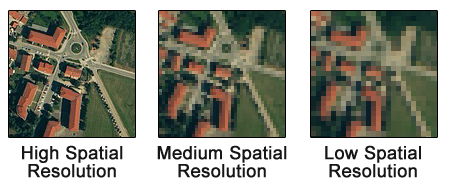
\includegraphics{images/Spatial-Resolution-Comparison.png}
\caption{spatial resolution comparsion}
\end{figure}

\hypertarget{temporal-resolution}{%
\subsection{\texorpdfstring{\textbf{Temporal resolution}}{Temporal resolution}}\label{temporal-resolution}}

Same definition of temporal resolution can be applied to polar orbiting satellites. But defining it more precisely, temporal resolution for a polar orbiting satellite is the amount of time that the satellite takes to revisit and recapture a particular site. It is also commonly referred to as a satellite's revisit period.

\begin{figure}
\centering
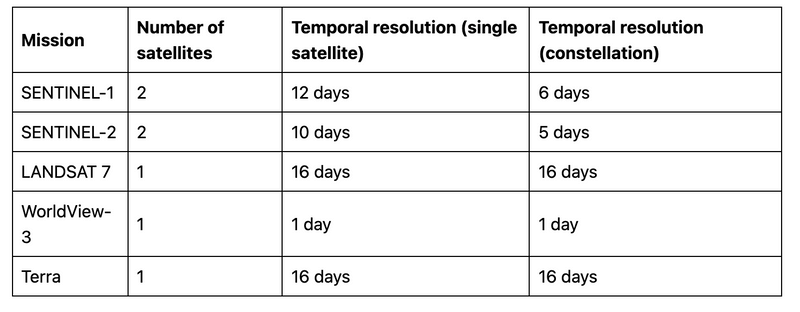
\includegraphics[width=0.95\textwidth,height=\textheight]{images/temporal-resolution.png}
\caption{Temporal resolution of some popular satellites}
\end{figure}

\hypertarget{spectral-resolution}{%
\subsection{\texorpdfstring{\textbf{Spectral resolution}\\
}{Spectral resolution }}\label{spectral-resolution}}

Spectral resolution is determined by the width of each band in a wavelength. The more bands in an image, the more complex the color will be.

\begin{figure}
\centering
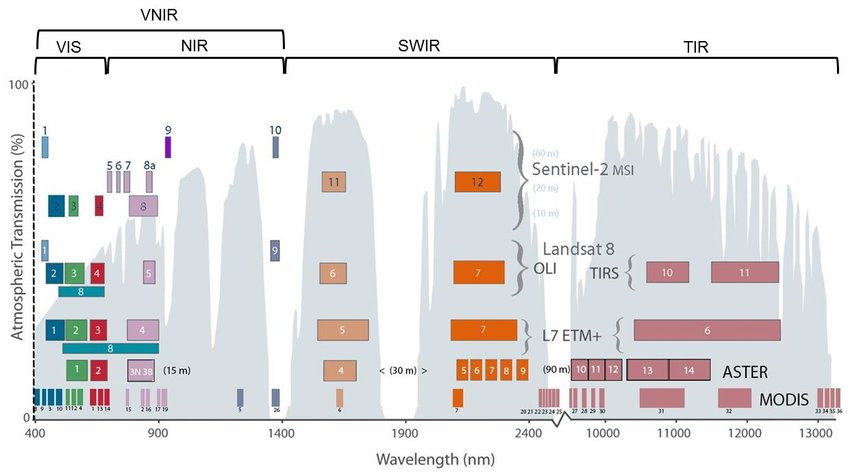
\includegraphics[width=0.9\textwidth,height=\textheight]{images/Spectral-resolution.png}
\caption{Spectral resolution of currently available optical satellite sensors grouped by different domains of the electromagnetic spectrum (VIS = visible, NIR = near infrared, VNIR = visible near infrared, SWIR = shortwave infrared, TIR = thermal infrared)}
\end{figure}

\hypertarget{crs}{%
\section{CRS}\label{crs}}

A Coordinate reference system (CRS) defines, with the help of coordinates, how the two-dimensional, projected map is related to real locations on the earth. There are two different types of coordinate reference systems: \textbf{\texttt{Geographic\ Coordinate\ Systems}} and \textbf{\texttt{Projected\ Coordinate\ Systems}}. CRS is very important for becoming a back-end developer of GIS.

\hypertarget{manipulation-in-r}{%
\section{Manipulation in R}\label{manipulation-in-r}}

How can we manipulate remote sensing imagery in R after we have a general understanding of raster data? Here I want to introduce to you a package: \texttt{terra}, which is a tweaked version or even a more powerful package than the well-known one: \texttt{raster}. As for the reason why the author choose to rebuild some functions, you can check it \href{http://www.wvview.org/os_sa/15_Raster_Analysis_terra.html}{here}.

\hypertarget{reference}{%
\section{Reference}\label{reference}}

\begin{itemize}
\tightlist
\item
  \url{http://modern-rstats.eu/index.html\#note-to-the-reader}
\end{itemize}

\hypertarget{multispectral-sensors}{%
\chapter{Multispectral sensors}\label{multispectral-sensors}}

In this section I'll introduce you to three well-known high-resolution multispectral sensor satellites in this section: \href{https://modis.gsfc.nasa.gov/}{MODIS}, \href{https://landsat.gsfc.nasa.gov/}{Landsat}, and \href{https://www.esa.int/Applications/Observing_the_Earth/Copernicus/Sentinel-2}{Sentinel-2}.

  \bibliography{book.bib,packages.bib}

\end{document}
